\documentclass[11pt]{article}
\usepackage[margin=1in]{geometry}
\usepackage{amsmath,amssymb,amsthm,mathtools}
\usepackage{dsfont}
\usepackage{graphicx}
\usepackage{booktabs}
\usepackage{array}
\usepackage{multirow}
\usepackage{placeins}
\usepackage[hyphens]{url}
\usepackage{microtype}
\usepackage{xcolor}
\usepackage{tikz}
\usetikzlibrary{arrows.meta,positioning,calc,decorations.pathreplacing}
\usepackage{caption}
\captionsetup{font=small,labelfont=bf,margin=0.5em}
\usepackage[colorlinks=true,linkcolor=blue!55!black,citecolor=blue!55!black,urlcolor=blue!55!black]{hyperref}

\newcommand{\Tr}{\operatorname{Tr}}
\newcommand{\Np}{N'}
\newcommand{\one}{\mathds 1}
\newcommand{\ip}[2]{\langle #1,#2\rangle}
\newcommand{\PH}{P_{\!H}}
\newcommand{\Om}{|\Omega\rangle}
\newcommand{\Zc}{\mathcal Z}
\newcommand{\Mb}{\mathbb M}
\newcommand{\SG}{\mathcal S_G}
\newcommand{\SGp}{\mathcal S'_G}
\newcommand{\sn}{s'}

% status tags (as in the previous reports)
\definecolor{cest}{RGB}{30,90,160}
\definecolor{cder}{RGB}{20,120,70}
\definecolor{cnum}{RGB}{150,90,10}
\definecolor{cconj}{RGB}{160,40,40}
\newcommand{\tagbox}[2]{\textsf{\small\color{#1}[#2]}}
\newcommand{\EST}{\tagbox{cest}{literature}}
\newcommand{\DER}{\tagbox{cder}{derived}}
\newcommand{\VER}{\tagbox{cder}{derived + verified}}
\newcommand{\NUM}{\tagbox{cnum}{numerical}}
\newcommand{\INTERP}{\tagbox{cconj}{interpretation}}

\theoremstyle{plain}
\newtheorem{theorem}{Theorem}
\newtheorem{proposition}{Proposition}
\newtheorem{corollary}{Corollary}
\theoremstyle{remark}
\newtheorem*{remark}{Remark}

\title{\bf Black holes dress, gravitons do not:\\ a chord picture of the two-flavor uplift\\[6pt]\large Progress report, 25 October 2026}
\author{\texttt{syk\_gravity} project\\[2pt]\small Drafted by Claude for J.~Chryssanthacopoulos; code at commit
\texttt{7f64254} (branch \texttt{t4-fourarc})}
\date{}

\emergencystretch=2em
\renewcommand{\topfraction}{0.9}
\renewcommand{\bottomfraction}{0.6}
\renewcommand{\textfraction}{0.08}
\renewcommand{\floatpagefraction}{0.8}
\numberwithin{equation}{section}

\begin{document}
\maketitle

\begin{abstract}
\noindent
The report of 23 October solved the BPS uplift of the symmetrized two-flavor $\mathcal N=2$ SYK model exactly. It found
that the monotone tower $V^n\Om$ is lifted bare at every $N$, while fortuitous states are dressed. Here we give the
double-scaled chord (``gravitational'') description of the same uplift, and find the distinction again, now in chord
language.
\begin{enumerate}\itemsep1pt
\item \emph{Two-flavor chords.} Repeating the chord derivation of Berkooz--Brukner--Narovlansky--Raz with two flavors
reduces the model to the one-flavor $\mathcal N=2$ chord theory, at $\lambda=2(p_\psi^2+p_\chi^2)/N=10/N$ and effective
charge $s=(2\delta N_\psi-\delta N_\chi)/5$. The uplift operators $\psi^\dagger\chi$, $\psi^\dagger\psi^\dagger$ and
$\psi^\dagger$ become chiral matter chords with $\delta=3/5,\,4/5,\,2/5$. The symmetrization that creates the tower adds
\emph{twisted chords}. These are suppressed by $1/N$ in every black-hole quantity, and they reduce to an insertion of the
graviton operator $V$.
\item \emph{The black-hole window.} BPS black holes, i.e.\ zero-length wormholes, live only in the window $|s|<1/2$. In the chord
theory its edges are gapless: they are the $Q=\pm\tfrac12$ supermultiplet of the $\mathcal N=2$ super-Schwarzian. In
the finite model the edge gap falls to $\sim\!4\times10^{-5}$ of the mean energy by $N=7$ and then stalls. Every BPS sector at
$\Np\le8$ lies in the window, except the outer tower sectors $(n,n)$. At $\Np=9$ the only BPS states outside the window
are tower states. In sector $(1,1)$ this is also the first place where the symmetrized and generic BPS dimensions
differ.
\item \emph{Uplift as emission.} Uplifting a black-hole state emits matter chords into the window's continuum. Without
fitted parameters, the Al-Salam--Chihara measures of these chords give the obstruction weights to 5--20\%, and the
dressing integrals to within a factor of about 1.4. When the uplift currents land on a gapless edge, at new charge
$\sn=\pm1/5$, the chord dressing diverges. The exact dressing in those sectors is resonantly enhanced by one to two orders of
magnitude in the mean (and up to four in the maximum) at $\Np=8$, in both models. This explains the nearly singular
dressing systems the 23 October report found at $\Np=8$.
\item \emph{Gravitons do not dress.} Taken one at a time, the tower's emissions are as large as the black holes', including
at the resonance. They cancel identically. The cancelling term is a twisted chord, i.e.\ a $V$ insertion, and it is
coherent only on $V$-descendants of the vacuum. The tower also absorbs the new flavor pair as a bound pair. Black holes
absorb its two fermions independently.
\end{enumerate}
\end{abstract}

\tableofcontents

%=====================================================================
\section{Introduction}\label{sec:intro}
%=====================================================================

\subsection{Where we stood}

The parent paper of Chryssanthacopoulos and Vegh (CV) \cite{CV} studied ``following $N$'' in $\mathcal N=2$ SYK through
the metric of the BPS space. It found that BPS states of the symmetrized two-flavor model of Chang, Chen, Sia and Yang
(CCSY) \cite{CCSY} split by how they lift from $N$ to $N+1$:
\begin{itemize}\itemsep1pt
\item the monotone tower $V^n\Om$, $V=\sum_i\psi_i^\dagger\chi_i^\dagger$, has a protected uplift;
\item the fortuitous states have dressing costs that grow with $N$.
\end{itemize}
CV closed by asking for ``a gravitational construction'' of this contrast.

The report of 23 October \cite{prog1023} solved the two-flavor uplift exactly. It wrote $Q_{N+1}=Q_0+\psi_e^\dagger
E+K\chi_f+\psi_e^\dagger Z\chi_f$, with
\begin{equation}
E=\textstyle\sum_{ik}(C_{eik}-C_{iek})\psi_i^\dagger\chi_k,\qquad
K=\textstyle\sum_{i<j}(C_{ijf}-C_{jif})\psi_i^\dagger\psi_j^\dagger,\qquad
Z=\textstyle\sum_i(C_{eif}-C_{ief})\psi_i^\dagger ,
\end{equation}
and decomposed a new BPS state into slots by the occupations $T=(t_\psi,t_\chi)$ of the new pair:
$\Psi=\Psi_{00}+\psi_e^\dagger\Psi_{10}+\chi_f^\dagger\Psi_{01}+\psi_e^\dagger\chi_f^\dagger\Psi_{11}$.
The uplift is then controlled by two currents,
\begin{equation}\label{eq:currents}
J_{10}=E\Psi_{00}-K\Psi_{11}+Z\Psi_{01},\qquad J_{01}=K^\dagger\Psi_{00}+E^\dagger\Psi_{11}+Z^\dagger\Psi_{10}.
\end{equation}
The dressing of a state is built from the time-integrated two-point functions of $E$, $K$ and $Z$ in the old model,
$G=H_0^+=\int_0^\infty d\tau\,(e^{-\tau H_0}-\PH)$.

The tower is \emph{bare}: $E V^n\Om=nKV^{n-1}\Om$ follows from the Ward identity $[E,V]=K$, so both currents vanish.
Fortuitous states are dressed. The 23 October report listed what a chord computation would have to supply: these two-point
functions, their mixed versions, and the transfer and leak maps of its closed form.

\subsection{What this report does}

We build the chord description of the two-flavor model and read the uplift in it. The aim is the one set in CV: see the
monotone/fortuitous contrast in a purely gravitational, i.e.\ chord, language. It appears there in three forms.

\begin{enumerate}\itemsep2pt
\item \textbf{Where} (\S\ref{sec:window}).
  \begin{itemize}\itemsep1pt
  \item The chord theory has BPS states only in the window $|s|<1/2$. These are BLY's zero-length wormholes, i.e.\ black
    holes.
  \item Fortuitous states live there.
  \item The tower lives on the diagonal $N_\psi=N_\chi$, which crosses the window and leaves it.
  \item Outside, from $\Np=9$ on, the tower is the only BPS state of its sector (up to boundary effects at the edge of
    charge space), and the continuum there is gapped. It is a horizonless state \INTERP.
  \end{itemize}
\item \textbf{How it lifts} (\S\ref{sec:emission}, \S\ref{sec:tower}).
  \begin{itemize}\itemsep1pt
  \item A black hole lifts by emitting matter chords into the window's continuum. The cost is a chord two-point
    function, and it diverges at the window's gapless edges.
  \item The tower emits nothing. Its emissions are as large as a black hole's and cancel through a twisted chord, the chord
    image of the graviton $V$.
  \end{itemize}
\item \textbf{How it absorbs the new pair} (\S\ref{sec:pairing}).
  \begin{itemize}\itemsep1pt
  \item Black holes absorb $\psi_e$ and $\chi_f$ independently (the chord weights factorize by flavor).
  \item The tower absorbs them as a bound pair.
  \end{itemize}
\end{enumerate}

Numerical checks use the exact finite-$N$ model at $\Np=N+1\le10$. They cover the symmetrized model and the generic
(Heydeman--Turiaci--Zhao \cite{HTZ}) control, with the realizations of \cite{prog1023}. Status tags: \EST, \DER,
\VER, \NUM, \INTERP. Plain-text record: \texttt{docs/derivations.md}, entry D9.

%=====================================================================
\section{Chords for two flavors}\label{sec:chords}
%=====================================================================

\subsection{The dictionary}

None of the papers in our collection treats the two-flavor model with chords. CCSY~\S3.3 and HTZ~\S3 use the large-$N$
$G$--$\Sigma$ method. We therefore derive the chord rules. Let every term of $Q$ create $p_\psi$ $\psi$'s and annihilate
$p_\chi$ $\chi$'s:
\[
Q=\sum_{I,K}C_{IK}\Psi_I^\dagger X_K,\qquad |I|=p_\psi,\ |K|=p_\chi .
\]
Our model has $p_\psi=2$, $p_\chi=1$. Take the double-scaling limit $p_\psi,p_\chi\to\infty$ at fixed ratio, with
$\lambda=2(p_\psi^2+p_\chi^2)/N$ fixed, and write $A=N_\psi-N/2$, $B=N_\chi-N/2$.

\begin{proposition}[two-flavor chords]\label{prop:dict}\DER\
The normalized moments of $H$ in the sector $(N_\psi,N_\chi)$ equal the fixed-charge chord moments of the one-flavor
$\mathcal N=2$ model (BBNR \cite{BBNR} eq.~(4.27)), at
\begin{equation}\label{eq:dict}
q=e^{-\lambda},\qquad \lambda=\frac{2(p_\psi^2+p_\chi^2)}{N},\qquad
s=\frac{p_\psi A-p_\chi B}{p_\psi^2+p_\chi^2}\quad\Big(=\frac{2A-B}{5},\ \ \lambda=\frac{10}N\ \text{ for our model}\Big).
\end{equation}
$Q$ raises $s$ by exactly~1.
\end{proposition}

\begin{proof}[Derivation]
We follow BBNR \S\S4.1--4.5 step by step.
\begin{enumerate}\itemsep2pt
\item \emph{Wick contraction.} Wick contraction gives oriented chord diagrams, each chord joining a $Q$ (an O-node) to a
  $Q^\dagger$ (an X-node) with the same $(I,K)$.
\item \emph{Pairs of chords.} For two chords, the overlaps $m_\psi=|I_1\cap I_2|$ and $m_\chi=|K_1\cap K_2|$ are
  independent: Poisson with means $p_\psi^2/N$ and $p_\chi^2/N$.
  \begin{itemize}\itemsep1pt
  \item \emph{Enemies} (BBNR (4.4i,ii)). A shared site would carry two $\psi^\dagger$'s, or two $\chi$'s, with nothing in
    between, so enemies need $m_\psi=m_\chi=0$. Weight $e^{-(p_\psi^2+p_\chi^2)/N}=q^{1/2}$.
  \item \emph{Friends.} Each shared site of either flavor gives a factor~2 (BBNR (4.6)--(4.7)). Weight
    $\mathbb E\,2^{m_\psi+m_\chi}=q^{-1/2}$.
  \item \emph{Crossings.} A term contains $p_\psi+p_\chi$ fermions (odd here), so crossings carry $(-1)^{\#\rm int}$.
  \end{itemize}
  This is BBNR (4.10) with the combined $\lambda$.
\item \emph{Chemical potentials.} Insert $e^{-\mu_\psi A-\mu_\chi B}$. A $\psi$-site carries $\psi^\dagger$ at the
  O-end of its chord, while a $\chi$-site carries $\chi$ there.
  \begin{itemize}\itemsep1pt
  \item At the base point of the trace, a right-pointing chord therefore leaves its $\psi$-sites occupied and its
    $\chi$-sites empty. A left-pointing chord does the reverse.
  \item Each chord contributes $e^{\mp(p_\psi\mu_\psi-p_\chi\mu_\chi)/2}$. Only $\mu_{\rm eff}=p_\psi\mu_\psi-p_\chi\mu_\chi$
    couples to the net orientation $m=n_\to-n_\leftarrow$.
  \item Sites outside all chords give $\cosh(\mu_\psi/2)^{N-kp_\psi}\cosh(\mu_\chi/2)^{N-kp_\chi}$. Doubly covered sites
    are subleading (BBNR's case~3).
  \end{itemize}
\item \emph{Fixed charge.} Fourier transforming in $(i\mu_\psi,i\mu_\chi)$ gives two Gaussian integrals, with result
  $e^{-2(A^2+B^2)/N}\,e^{\lambda sm}\,e^{-\lambda m^2/4}$.
  \begin{itemize}\itemsep1pt
  \item The first factor is the sector-dimension fraction.
  \item The last cancels BBNR's $q^{-m^2/4}$ of (4.14), because both involve the same combined $\lambda$.
  \end{itemize}
  What remains is BBNR (4.24)--(4.27) at charge~$s$.\qedhere
\end{enumerate}
\end{proof}

\paragraph{Matter.} Consider a matter operator $O=\sum\eta_{I'K'}\Psi_{I'}^\dagger X_{K'}$ with independent Gaussian
couplings, $|I'|=p'_\psi$ and $|K'|=p'_\chi$.
\begin{itemize}\itemsep1pt
\item An $H$-chord crossing it overlaps it in Poisson$(p_\psi p'_\psi/N)$ $\psi$-sites and Poisson$(p_\chi p'_\chi/N)$
  $\chi$-sites. The crossing weight is $q^\delta$, with
  \begin{equation}\label{eq:delta}
  \delta=\frac{p_\psi p'_\psi+p_\chi p'_\chi}{p_\psi^2+p_\chi^2}.
  \end{equation}
\item $O$ shifts $s$ by the same $\delta$. It is therefore a \emph{chiral} single-chord operator in the sense of the
  14 October report \cite{prog1014}: its charge shift equals its crossing exponent.
\item For the uplift operators,
  \begin{equation}\label{eq:deltas}
  E=\psi^\dagger\chi:\ \delta=\tfrac35,\qquad K=\psi^\dagger\psi^\dagger:\ \delta=\tfrac45,\qquad Z=\psi^\dagger:\ \delta=\tfrac25 .
  \end{equation}
  Their adjoints lower $s$ by the same amounts. They are mapped to raising operators by the mirror $s\to-s$.
\end{itemize}

\paragraph{Chirality is exact here.} $Q_0$, $E$, $K$ and $Z$ are polynomials in the mutually anticommuting set
$\{\psi_i^\dagger,\chi_k\}$. Hence, identically,
\begin{equation}\label{eq:chiral}
[Q_0,E]=[Q_0,K]=[E,K]=0,\qquad \{Q_0,Z\}=0
\end{equation}
(checked to $10^{-15}$). So for a BPS state $h$, $Oh$ is $Q_0$-closed: it lies in BPS $\oplus$ exact, which is the
``B family'' of the chord theory. Likewise $O^\dagger h$ lies in BPS $\oplus$ coexact. This is exactly the support that the
chord spectral measure assigns.

\begin{remark}
The 23 October report derived $[E,K]=\{Q_0,Z\}$ from nilpotency. By \eqref{eq:chiral} both sides vanish. No result there
depended on the identity being nontrivial. In particular $\{Q_0,\Zc\}=E\PH K-K\PH E$ for $\Zc=Z-EQ_0^+K+KQ_0^+E$ is
unaffected.
\end{remark}

\subsection{Twisted chords: what the symmetrization does}\label{sec:twisted}

The tower needs couplings symmetric in the second $\psi$-index and the $\chi$-index, $C_{ijk}=C_{ikj}$. The
antisymmetrized couplings $A_{ijk}=C_{ijk}-C_{jik}$ of $C=(G+G^{T_{jk}})/2$ (with $\mathbb E|G|^2=2$) then have covariance
\begin{equation}\label{eq:twisted}
\langle A_{ijk}\bar A_{lmn}\rangle=(\delta_{il}\delta_{jm}-\delta_{im}\delta_{jl})\delta_{kn}
+\tfrac12\big[\delta_{il}\delta_{jn}\delta_{km}-\delta_{im}\delta_{jn}\delta_{kl}-\delta_{jl}\delta_{in}\delta_{km}+\delta_{jm}\delta_{in}\delta_{kl}\big].
\end{equation}
\begin{itemize}\itemsep1pt
\item The first term is the ordinary chord.
\item The bracket joins a $Q$-term to a $Q^\dagger$-term in which a $\psi$-index and the $\chi$-index are exchanged: a
  \emph{twisted chord}.
\item Written out, $\psi_i^\dagger\psi_j^\dagger\chi_k\cdots\chi_j^\dagger\psi_k\psi_i$ is a number factor on site $i$
  times $\psi_j^\dagger\chi_j^\dagger$ times $\chi_k\psi_k$. A twisted chord \emph{moves a $\psi\chi$ pair} from site $k$ to
  site $j$.
\end{itemize}

\begin{proposition}[twisted chords]\label{prop:twisted}\DER\ (counting)
\begin{enumerate}\itemsep1pt
\item In a trace, or a diagonal matrix element in a Fock state, twisted chords cost a factor $1/N$ each. This includes
  densities of states, BPS fractions, and BPS-averaged correlators of operators with independent couplings. At leading
  order the symmetrized and generic models have the same chord diagrams.
\item On the states $V^n\Om=\sum_{|S|=n}\prod_{i\in S}\psi_i^\dagger\chi_i^\dagger\Om$, twisted chords act coherently and
  are $O(1)$.
\item The $E$--$K$ cross-covariance of the symmetrized model is a twisted matter chord whose net effect is a $V$
  insertion.
\end{enumerate}
\end{proposition}

\begin{proof}[Argument]
\emph{(1)} In a trace every mode must balance, so the pair hops of the twisted chords in a diagram must compose to the
identity. For $t$ twisted chords this costs at least $t$ index identifications beyond an untwisted diagram ($j=k$ for
$t=1$), each worth $1/N$.

\emph{(2)} On $V^n\Om$, a hop maps tower configurations to tower configurations with equal amplitude. The sum over the
$N^2$ hops is therefore coherent, and no identification is needed.

\emph{(3)} In the symmetrized model $K_{ij}=E_{ji}-E_{ij}$ (the protection identity of \cite{prog1023}, its \S2.2). Hence
$\mathbb E[\bar E_{i'k'}K_{ij}]=v(\delta_{i'j}\delta_{k'i}-\delta_{i'i}\delta_{k'j})$. In a cross term such as
$\ip{E h}{G K h'}$, $K$ creates $\psi_i^\dagger$ and $E^\dagger$ creates $\chi_i^\dagger$ at the same site. The net effect is
$\psi_i^\dagger\chi_i^\dagger$ summed over $i$, i.e.\ $V$.
\end{proof}

Item~(1) is the chord-level version of CCSY \S3.3, which found that symmetrization leaves the $G$--$\Sigma$ action
unchanged. Here it holds for all moments and correlators, not only for the saddle. It is consistent with what the 23
October report found numerically: the BPS dimensions and both room laws coincide in the two models for $\Np\le8$.

%=====================================================================
\section{The black-hole window}\label{sec:window}
%=====================================================================

\subsection{Where BPS black holes live}

\paragraph{The window.} \EST+\DER\ In the window $|s|<1/2$, the chord BPS fraction
$D(s)=(q^{1+2s},q^{1-2s},q^2;q^2)_\infty$ (BLY \cite{BLY} eq.~(3.17)) is the probability of a zero-length wormhole. It
vanishes at the edges $s=\pm\tfrac12$. Outside the window there are no ground states: the exact count, BBNR (5.25), is
nonzero only for $|s|<\tfrac12$.
\begin{itemize}\itemsep1pt
\item Since $Q$ shifts $s$ by 1, a $Q$-complex has at most one window sector. This is CCSY's R-charge concentration in
  double-scaled form.
\item In charge space, by \eqref{eq:dict}, the window is the band
  \begin{equation}\label{eq:band}
  \big|\,2(N_\psi-\tfrac N2)-(N_\chi-\tfrac N2)\,\big|<\tfrac52 .
  \end{equation}
  It has slope $dN_\chi/dN_\psi=2$ through the center.
\end{itemize}

\paragraph{Comparison with CCSY.} \NUM\ CCSY derive a nonlinear charge constraint at large $N$ and fixed
$p=(2,1)$ (their eq.~(3.14)). Evaluated here, it passes through the center with slope $dn_\chi/dj=0.392$ (where $j=n_\psi+2n_\chi$).
The band~\eqref{eq:band} has $2/5$. So the band is the double-scaled linearization of CCSY's line, and the 2\% slope
difference is a finite-$p$ effect. At $N\le10$ it shifts the band by at most about 0.2 of a sector, except at the boundary
of charge space.

\paragraph{The tower relative to the window.} The tower sector $(n,n)$ has $s=(n-N/2)/5$. It lies inside the window if
and only if $|n-N/2|<5/2$. Following $N$ at fixed $n$, the tower crosses the window in about ten uplifts and then stays
BPS outside it, where the chord theory has no BPS states.

\subsection{The edges are gapless}

\DER\ By BBNR (5.3), with the sign fixed in the 14 October report \cite{prog1014}, the continua at charge $s$ begin at
\begin{equation}\label{eq:edges}
E_B(s)=2q^{-1/2}\kappa\,[\cosh\lambda(s-\tfrac12)-1],\qquad E_A(s)=2q^{-1/2}\kappa\,[\cosh\lambda(s+\tfrac12)-1].
\end{equation}
Here $B$ is the exact family and $A$ the coexact one. So the exact continuum reaches zero energy at $s=+\tfrac12$, and the
coexact continuum at $s=-\tfrac12$. Near such an edge the B-family density in $\phi$ tends to a constant while
$\Lambda\propto\phi^2$, so $\rho(E)\propto E^{-1/2}$: a hard edge.

\INTERP\ This is the near-BPS black-hole spectrum of the $\mathcal N=2$ super-Schwarzian.
\begin{itemize}\itemsep1pt
\item There, the supermultiplet of R-charge $Q$ has its continuum starting at $E_0(Q)=(Q-\tfrac12)^2/(8\Phi_r)$, and BPS
  states exist only for $|Q|<\tfrac12$ (Heydeman--Iliesiu--Turiaci--Zhao \cite{HITZ}, App.~A, eqs.~(A.14), (A.18)).
\item Whether there is a gap depends on whether the charge lattice contains $Q=\tfrac12$: ``there is no gap since for
  $Q=1/2$, $E_0(1/2)=0$'' (\cite{HITZ}, App.~A and Fig.~5).
\item \eqref{eq:edges} is the finite-$\lambda$ form of $E_0$.
\item For our model, $s\in\tfrac15\mathbb Z$ at even $N$ and $s\in\tfrac15\mathbb Z+\tfrac1{10}$ at odd $N$. So odd $N$
  has the gapless supermultiplet on its charge lattice, and even $N$ does not.
\item The two edges are the two halves of one multiplet. $Q$ maps the coexact family at $s=-\tfrac12$ onto the exact family
  at $s=+\tfrac12$ of the same complex, and the two share their nonzero spectrum. At $N=7$, for example, $(2,3)\to(4,2)$ carries
  the near-zero level $0.003175$ in both sectors.
\end{itemize}

\subsection{Tests}\label{sec:windowtests}

\NUM\ We use exact BPS dimensions, fractions and gaps:
\begin{itemize}\itemsep1pt
\item every sector at $\Np=4$--8 (both models; seeds 1--3, and 1--2 at $\Np=8$);
\item every sector of dimension $\le3000$ at $\Np=9,10$ (seeds 1--2).
\end{itemize}
See Figs.~\ref{fig:window} and~\ref{fig:dict}c.

\begin{itemize}\itemsep2pt
\item \emph{Support.} At $\Np=4$--8 every sector with BPS states lies in $|s|\le\tfrac12$, except diagonal (tower)
  sectors $(n,n)$ with $|n-\Np/2|\ge3$.
  \begin{itemize}\itemsep1pt
  \item At $\Np=4$--7 these are $(0,0)$ and $(\Np,\Np)$, the vacuum and the filled state.
  \item At $\Np=8$ they are also $(1,1)$ and $(7,7)$, at $s=\mp0.6$. Each holds 8 states: the tower plus 7 forced by
    dimension counting ($\dim(1,1)=64>\dim(3,0)=56$). The in-window partners of these two complexes, $(3,0)$ and $(5,8)$,
    are then empty.
  \end{itemize}
\item \emph{Only monotone states outside.} At $\Np=9$ every BPS state strictly outside the window (in the sectors computed)
  is a tower state: one each in $(0,0)$, $(1,1)$, $(8,8)$ and $(9,9)$. At $\Np=10$ two kinds of monotone state appear:
  \begin{itemize}\itemsep1pt
  \item the tower;
  \item CCSY's ``exposed-index'' monotone states $\psi_i^\dagger\Om$ (their eq.~(3.9)), which fill $(1,0)$ and $(9,10)$ at
    $s=\mp0.6$.
  \end{itemize}
  The one exception is the boundary complex discussed below.
\item \emph{The tower alone.} At $\Np=9,10$ counting no longer forces states into $(1,1)$ ($81<84$, $100<120$).
  \begin{itemize}\itemsep1pt
  \item The symmetrized model has exactly one BPS state there, the tower. The generic model has none (both seeds).
  \item This is the first sector where the BPS dimensions of the two models differ. The 23 October report found them
    equal at $\Np\le8$.
  \end{itemize}
\item \emph{A boundary miss.} At $\Np=10$ the 15 BPS states of the complex $J=N_\psi+2N_\chi=6$ sit in $(2,2)$, at
  $s=-0.6$, just outside the band, in both models. With symmetrized couplings one of the 15 is the tower. This is the
  curvature of CCSY's line near the boundary of charge space.
\item \emph{Fractions.} Over window sectors of dimension $\ge20$, exact$/D(s)$ averages 0.91--1.04, with range 0.79--1.76
  (excluding the two empty boundary sectors $(3,0)$ and $(5,8)$ at $\Np=8$).
  In central sectors it is 0.84--0.95 (Fig.~\ref{fig:window}c). In the one-flavor model at $p=3$ the comparison gave
  0--10\%; here $p_\chi=1$.
\item \emph{Continuum edges.} In bulk sectors off the edge (dimension $\ge50$), the exact lowest eigenvalue of each family
  divided by the chord edge~\eqref{eq:edges} has geometric mean 0.65--0.97 and log-scatter 0.2--0.47, over gaps spanning
  three decades (Fig.~\ref{fig:dict}c). The exact gaps are systematically somewhat lower, as in the one-flavor model.
\item \emph{Gapless edges.} In window-edge sectors of large dimension, the predicted gapless family reaches down to
  about $5\times10^{-5}$ of the sector's mean energy at $N=7$. The bulk median is 0.06--0.12. The lowest levels accumulate:
  at $N=7$ the six lowest lie between $7\times10^{-5}$ and $3\times10^{-4}$ of the mean.
\end{itemize}

\begin{figure}[t]
\centering
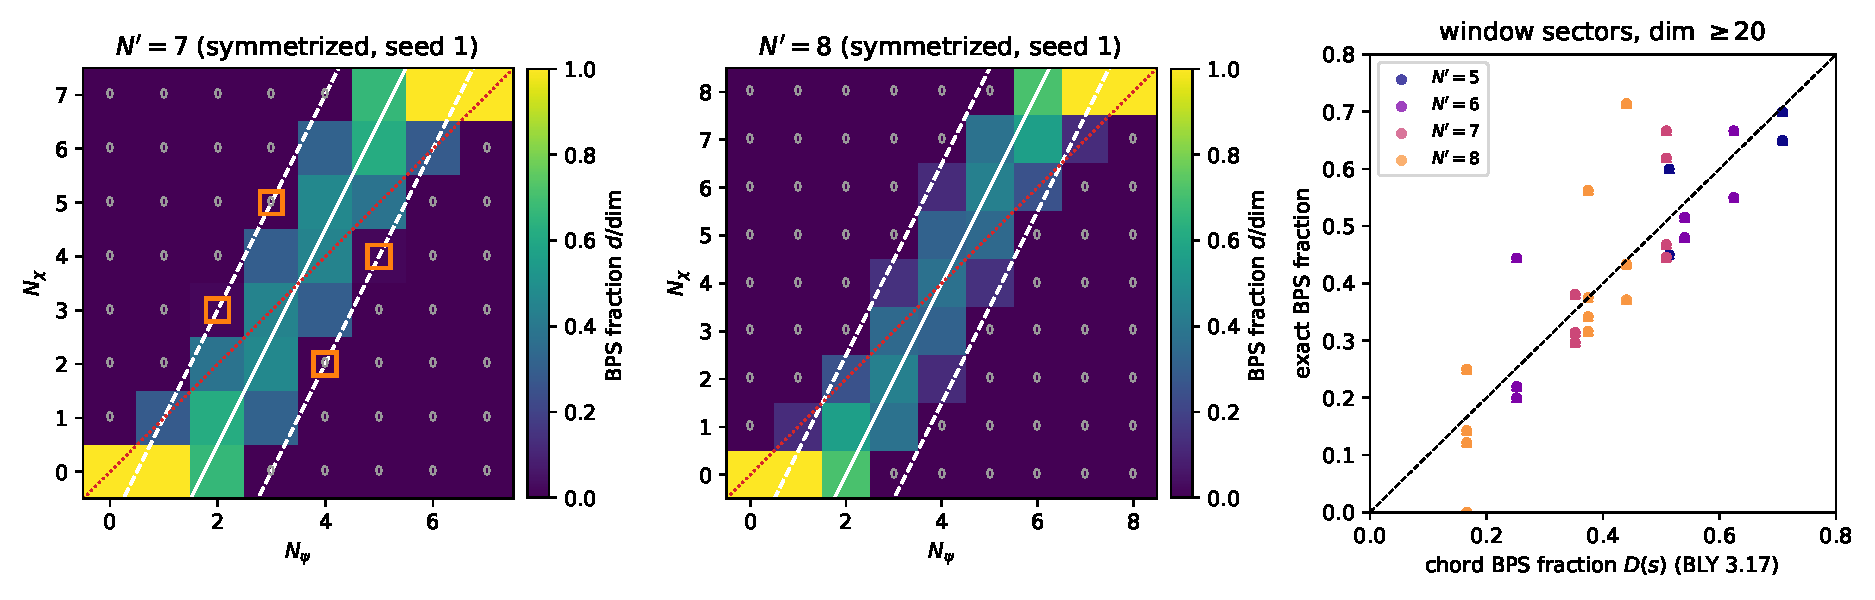
\includegraphics[width=\textwidth]{progress_2026-10-25_figs/fig_window.pdf}
\caption{\textbf{The black-hole window.} (a, b) Exact BPS fraction by sector at $\Np=7,8$ (symmetrized, seed~1).
The white lines are the band \eqref{eq:band}: $s=0$ (solid) and $s=\pm\tfrac12$ (dashed). The red dotted line is the
tower diagonal. Orange squares mark window-edge sectors whose predicted gapless family has a gap below $10^{-2}$ of the mean
energy; ``0'' marks sectors without BPS states. (c) Exact BPS fraction against the chord value $D(s)$ (BLY 3.17) for window
sectors of dimension $\ge20$. Circles: symmetrized; triangles: generic.}
\label{fig:window}
\end{figure}

%=====================================================================
\section{The uplift as emission into the window}\label{sec:emission}
%=====================================================================

\subsection{Bookkeeping}

Take a new BPS state in sector $(A,B)$ of the $\Np$-model, at chord charge $\sn=s_{\Np}(A,B)$. By \eqref{eq:dict} with
$p=(2,1)$, its old slots sit at $\sn+\tfrac1{10}$ (00), $\sn-\tfrac1{10}$ (11), $\sn-\tfrac3{10}$ (10) and
$\sn+\tfrac3{10}$ (01). The six first-order dressing terms of \cite{prog1023} land as follows.

\begin{center}\small
\begin{tabular}{llll}
\toprule
term & sources & old target sector & target charge\\
\midrule
current $J_{10}$ & $Eh_{00}$, $Kh_{11}$, $Zh_{01}$ & $(A+1,B-1)$ & $\sn+\tfrac7{10}$ (raising)\\
current $J_{01}$ & $K^\dagger h_{00}$, $E^\dagger h_{11}$, $Z^\dagger h_{10}$ & $(A-2,B)$ & $\sn-\tfrac7{10}$ (lowering)\\
$z_{11}=-Q_0^+Eh_{01}$ & $Eh_{01}$ & $(A+1,B-2)$ & $\sn+\tfrac9{10}$\\
$x_{00}=-(Q_0^\dagger)^+E^\dagger h_{10}$ & $E^\dagger h_{10}$ & $(A-2,B+1)$ & $\sn-\tfrac9{10}$\\
$z_{00}=-Q_0^+Kh_{01}$ & $Kh_{01}$ & $(A+2,B-1)$ & $\sn+\tfrac{11}{10}$\\
$x_{11}=(Q_0^\dagger)^+K^\dagger h_{10}$ & $K^\dagger h_{10}$ & $(A-3,B)$ & $\sn-\tfrac{11}{10}$\\
\bottomrule
\end{tabular}
\end{center}

\begin{figure}[t]
\centering
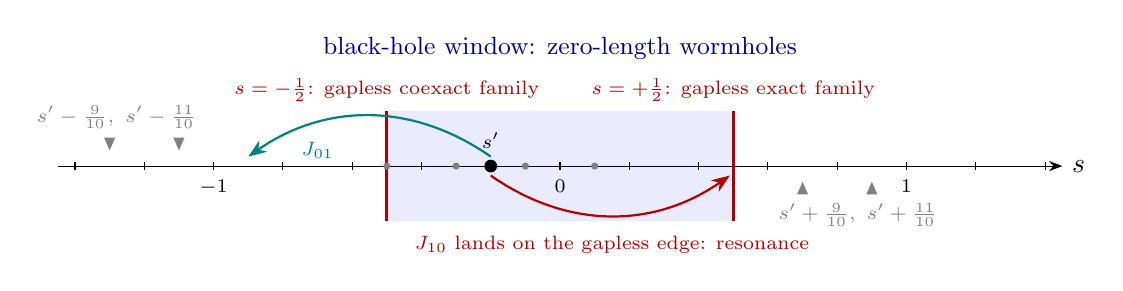
\begin{tikzpicture}[x=4.4cm,y=1cm,>=Stealth]
\fill[blue!8] (-0.5,-0.7) rectangle (0.5,0.7);
\draw[->] (-1.45,0) -- (1.45,0) node[right] {$s$};
\foreach \x in {-1.4,-1.2,...,1.41} \draw (\x,0.05) -- (\x,-0.05);
\foreach \x/\l in {-1/-1,0/0,1/1} \node[below] at (\x,-0.05) {\scriptsize $\l$};
\draw[very thick,red!70!black] (0.5,-0.7) -- (0.5,0.7);
\draw[very thick,red!70!black] (-0.5,-0.7) -- (-0.5,0.7);
\node[red!70!black,above] at (0.5,0.7) {\scriptsize $s=+\tfrac12$: gapless exact family};
\node[red!70!black,above] at (-0.5,0.7) {\scriptsize $s=-\tfrac12$: gapless coexact family};
\node[blue!60!black] at (0,1.5) {\small black-hole window: zero-length wormholes};
\fill (-0.2,0) circle (2.3pt); \node[above] at (-0.2,0.1) {\scriptsize $s'$};
\foreach \x in {-0.1,-0.3,-0.5,0.1} \fill[gray] (\x,0) circle (1.3pt);
\draw[->,thick,red!70!black] (-0.2,-0.12) to[bend right=35] (0.49,-0.12);
\node[red!70!black] at (0.15,-1.0) {\scriptsize $J_{10}$ lands on the gapless edge: resonance};
\draw[->,thick,teal] (-0.2,0.12) to[bend right=35] (-0.9,0.12);
\node[teal] at (-0.7,0.2) {\scriptsize $J_{01}$};
\foreach \x in {0.7,0.9} \fill[gray] (\x,-0.2) -- ++(-0.016,-0.16) -- ++(0.032,0) -- cycle;
\foreach \x in {-1.1,-1.3} \fill[gray] (\x,0.2) -- ++(-0.016,0.16) -- ++(0.032,0) -- cycle;
\node[gray] at (0.86,-0.62) {\scriptsize $s'+\tfrac{9}{10},\ s'+\tfrac{11}{10}$};
\node[gray] at (-1.28,0.62) {\scriptsize $s'-\tfrac{9}{10},\ s'-\tfrac{11}{10}$};
\end{tikzpicture}
\caption{\textbf{The uplift on the $s$ line} ($p=(2,1)$). A new black-hole state at $\sn$ (black dot) has old slot
components at $\sn\pm\tfrac1{10},\pm\tfrac3{10}$ (gray dots). Its currents emit into the old continuum at $\sn\pm\tfrac7{10}$
(arrows). Its single-flavor slots emit at $\sn\pm\tfrac9{10},\pm\tfrac{11}{10}$ (triangles below the axis for raising terms,
above for lowering ones). Shown is $\sn=-\tfrac15$, where $J_{10}$ lands on the gapless exact-family edge at $s=+\tfrac12$.}
\label{fig:sline}
\end{figure}

\subsection{Emission spectra}

\DER\ (14 October report, D7 \S\S1--2.) Take a BPS state at charge $s_{\rm out}$ and a chiral operator raising the charge
by $\delta$ to $s_{\rm in}=s_{\rm out}+\delta$. Normalized to unit total weight, the spectral measure of the operator acting on
the state is the Al-Salam--Chihara (ASC) measure, with
\[
a=q^{s_{\rm in}-1/2},\qquad b=q^{1/2+\delta-s_{\rm out}} .
\]
\begin{itemize}\itemsep1pt
\item \emph{Point mass.} If $s_{\rm in}<\tfrac12$ the measure has a point mass at zero energy,
  \begin{equation}\label{eq:pm}
  \frac{\|\PH Oh\|^2}{\|Oh\|^2}=\frac{(q^{1-2s_{\rm in}};q^2)_\infty}{(q^{1-2s_{\rm out}};q^2)_\infty}
  \qquad\text{(BLY 4.14)} .
  \end{equation}
  This is the \emph{obstruction weight} of Theorem~1 of \cite{prog1023}, which now has a chord value.
\item \emph{Continuum.} The continuous part, integrated against $1/(\kappa\Lambda)$, gives the time-integrated two-point
  function. These are the dressing building blocks, in units of $c_0$, the exact $\tau=0$ value.
\end{itemize}
As in D7, $\kappa$ is fixed by the exact first moment of the target sector. There are no fitted parameters.

\NUM\ For every old sector and every one of $E$, $K$, $Z$ and their adjoints (with unit-variance independent
couplings, averaged exactly), we compare chord and exact values at $N=3$--7, in both models (Fig.~\ref{fig:dict}a,b).
\begin{itemize}\itemsep1pt
\item \emph{Obstruction weights:} chord/exact has geometric mean 1.05--1.21 and log-scatter 0.06--0.29.
\item \emph{Time integrals with targets at least 0.15 from an edge:} geometric mean 0.80--1.08, log-scatter 0.17--0.34.
  The values span two and a half decades.
  \begin{itemize}\itemsep1pt
  \item The mild drift to 0.80--0.88 at $N=7$ goes with the exact gaps lying below the chord edges (\S\ref{sec:windowtests}).
  \item Targets 0.1 from an edge give 0.89--0.96 with larger scatter (0.27--0.71).
  \end{itemize}
\item Both models agree equally well with the chords, as Proposition~\ref{prop:twisted}(1) requires.
\item \emph{Targets exactly on a large edge} (chord value $\infty$) give exact $T/c_0$ medians of 0.46--0.53 at $N=5$ and
  1.2--2.8 at $N=7$, against 0.011--0.062 off the edge. They are enhanced 25--250$\times$, and the enhancement grows with
  $N$.
\end{itemize}

\begin{figure}[t]
\centering
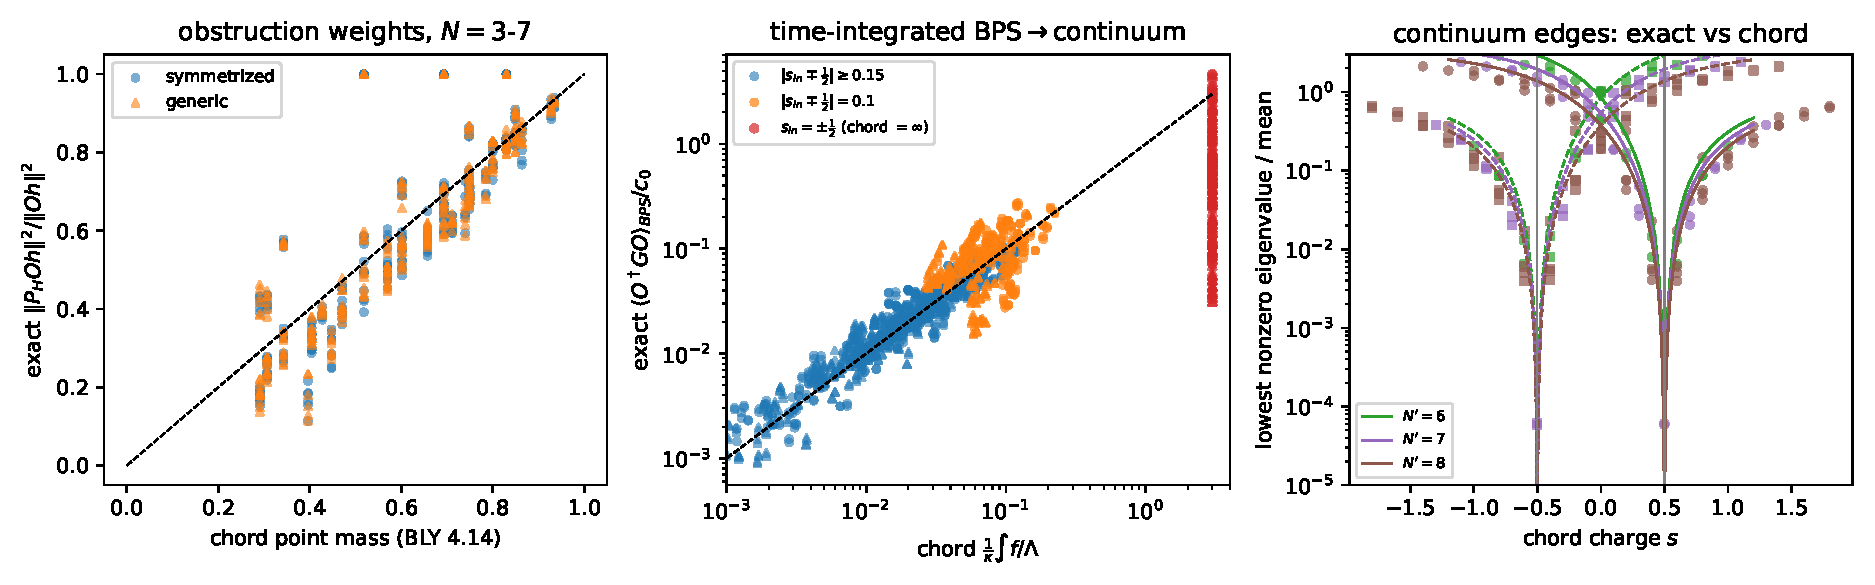
\includegraphics[width=\textwidth]{progress_2026-10-25_figs/fig_dictionary.pdf}
\caption{\textbf{The chord dictionary, tested.}
(a) Obstruction weight $\|\PH Oh\|^2/\|Oh\|^2$, BPS-averaged, exact vs the chord point mass \eqref{eq:pm}.
(b) Time-integrated BPS$\to$continuum two-point function per unit $c_0$, exact vs chord. Blue: targets at least 0.15 from
a gapless edge. Orange: 0.1 from it. Red, plotted at abscissa~3: targets exactly on an edge, where the chord value is
infinite.
(c) Lowest nonzero eigenvalue of the exact (circles) and coexact (squares) families divided by the sector's mean, vs $s$,
at $\Np=6,7,8$. Lines: the chord edges \eqref{eq:edges} (solid B, dashed A).}
\label{fig:dict}
\end{figure}

\subsection{Resonances}\label{sec:resonance}

\DER\ Suppose a term lands on its gapless edge: a raising term at $s_{\rm in}=+\tfrac12$, or a lowering term at
$-\tfrac12$. Then $a\to1$, so $f(\phi)\to$ const while $\Lambda\propto\phi^2$, and the chord time integral
$\int f/\Lambda\,d\phi\sim\int d\phi/\phi^2$ \emph{diverges}.
\begin{itemize}\itemsep1pt
\item From the table, the resonant new charges are $\sn=-\tfrac15$ ($J_{10}$), $-\tfrac25$ ($z_{11}$), $-\tfrac35$
  ($z_{00}$), and their mirrors.
\item For $p=(2,1)$, $\sn\in\tfrac15\mathbb Z$ at even $\Np$. So the \emph{currents are exactly resonant only at even
  $\Np$}, in the sectors $\sn=\pm\tfrac15$.
\item At odd $\Np$ every bulk sector is $\tfrac1{10}$ from an edge, i.e.\ near-resonant.
\end{itemize}
The chord prediction is that black-hole dressing grows as the emission approaches a gapless edge. At finite $N$ it is
controlled by the edge sector's near-zero modes.

\NUM\ The exact dressing $\kappa=1/\mu-1$ of every new BPS state, from the exact bare fraction $\mu$, is shown in
Fig.~\ref{fig:resonance} for both models.
Sectors are classified a priori: by whether a dressing term is resonant, and, if so, by the dimension of the edge sector
it lands in. Only bulk sectors (at least 30 new BPS states) are used. Each entry is the median over sectors of the
per-sector mean, or largest, dressing:
\begin{center}\small
\begin{tabular}{lcccc}
\toprule
 & \multicolumn{2}{c}{$\Np=6$ (seeds 1--3)} & \multicolumn{2}{c}{$\Np=8$ (seeds 1--2)}\\
\cmidrule(lr){2-3}\cmidrule(lr){4-5}
 & sym & generic & sym & generic\\
\midrule
$J$-resonant, large edge target: mean $\kappa$ & 4.8 & 9.8 & 125 & 48\\
\qquad largest $\kappa$ & 270 & 778 & $7.8\times10^4$ & $1.5\times10^4$\\
$J$-resonant, small boundary target: mean / largest & -- & -- & 1.3 / 35 & 1.2 / 31\\
$z$-resonant: mean / largest & 1.2 / 10 & 1.6 / 15 & 2.4 / 34 & 2.2 / 28\\
non-resonant: mean / largest & 0.42 / 6.7 & 0.51 / 7.9 & 1.0 / 30 & 0.98 / 29\\
\bottomrule
\end{tabular}
\end{center}
\begin{itemize}\itemsep2pt
\item \emph{Size.} At $\Np=8$ the $J$-resonance raises the mean dressing by a factor 50--125 and the largest by
  $10^3$--$10^4$, in both models.
\item \emph{Growth.} Between $\Np=6$ and 8 it grows by one to two orders of magnitude.
\item \emph{Tail.} Medians over states barely move (0.37--0.40 at $\Np=8$). The resonance lives in the upper tail, the
  states with a large overlap with the near-zero modes.
\item \emph{Control.} The ``small boundary target'' rows have the same resonant charge $\sn=\pm\tfrac15$, but their
  currents land in small edge sectors at the boundary of charge space, which have no black-hole continuum and no near-zero
  modes (e.g.\ $(3,0)$, of dimension 35). They show no enhancement. So the enhancement comes from the gapless
  continuum, not from the charge label.
\item \emph{Odd $\Np$.} Here every bulk sector is $\tfrac1{10}$ from an edge. At $\Np=7$ the mean is 1.8 and the largest
  44--55, in between.
\item \emph{Ordering.} Ordered by the distance of the currents' targets from the edge, the dressing falls monotonically
  (Fig.~\ref{fig:resonance}, right).
\end{itemize}
This explains a finding of \cite{prog1023}. Its closed-form dressing system was nearly singular at $\Np=8$, in $(3,3)$
and $(5,5)$, with an ``old gap 0.0032''. Both are $J$-resonant sectors ($\sn=\mp\tfrac15$). The old gap is the near-zero
mode of the edge sector $(4,2)$ at $N=7$: $0.003175$, i.e.\ $4.4\times10^{-5}$ of its mean energy.

\paragraph{How the edge gap scales.} \NUM\ (Task \texttt{edgegap}; Fig.~\ref{fig:edgegap}.) In the largest window-edge
sector, the lowest level of the predicted gapless family, relative to the sector's mean energy, is:
\begin{center}\small
\begin{tabular}{lcccc}
\toprule
$N$ & 3 & 5 & 7 & 9\\
family dimension $D$ & 3 & 48 & 686 & 9297\\
lowest level / mean & 0.05--0.27 & $4\times10^{-4}$--$4\times10^{-3}$ & $3\times10^{-5}$--$1\times10^{-4}$ & $3.3\times10^{-5}$--$4.8\times10^{-5}$\\
\bottomrule
\end{tabular}
\end{center}
\begin{itemize}\itemsep1pt
\item Up to $N=7$ the gap falls by about two orders of magnitude per step, faster than $D^{-1}$.
\item At $N=9$ it stalls, in both models and both seeds, while the levels above it pile up: the six lowest lie within a
  factor 1.4--1.55 of each other, against a factor 5 at $N=7$.
\item So the chord model's exact gaplessness is approached but not reached at $p=(2,1)$.
\end{itemize}
\INTERP\ A possible reading: the true gapless edge, CCSY's curved line in IR-charge terms, sits at $s=\tfrac12+\Delta s$,
slightly off the double-scaled value. The chord edge \eqref{eq:edges} then leaves a residual gap
$\approx\lambda^2\Delta s^2/(1+q)$ in these units. $\Delta s\approx0.006$ reproduces $N=9$ and is consistent with $N=7$; at
$N\le5$ the discreteness of the levels dominates instead. A fixed $\Delta s$ makes the residual gap fall only like
$\lambda^2\propto N^{-2}$, a factor 0.6 from $N=7$ to 9, as against the exponentially fast fall of the level spacing up
to $N=7$. This $\Delta s$ is fitted, and two points cannot fix a scaling, so the reading is a conjecture.

\begin{figure}[t]
\centering
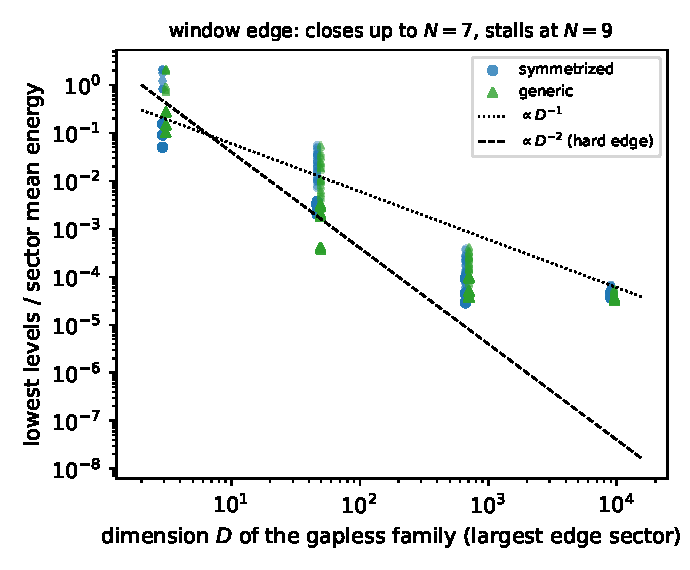
\includegraphics[width=0.5\textwidth]{progress_2026-10-25_figs/fig_edgegap.pdf}
\caption{\textbf{The window edge closes, then stalls.} Lowest (large marks) and next five (small marks) levels of the
chord-gapless family in the largest window-edge sector, divided by the sector's mean energy, against the family dimension
$D$, for $N=3,5,7,9$. Circles: symmetrized; triangles: generic. Guides: $D^{-1}$ (dotted) and $D^{-2}$ (dashed, a hard
edge with a fixed density).}
\label{fig:edgegap}
\end{figure}

\begin{figure}[t]
\centering
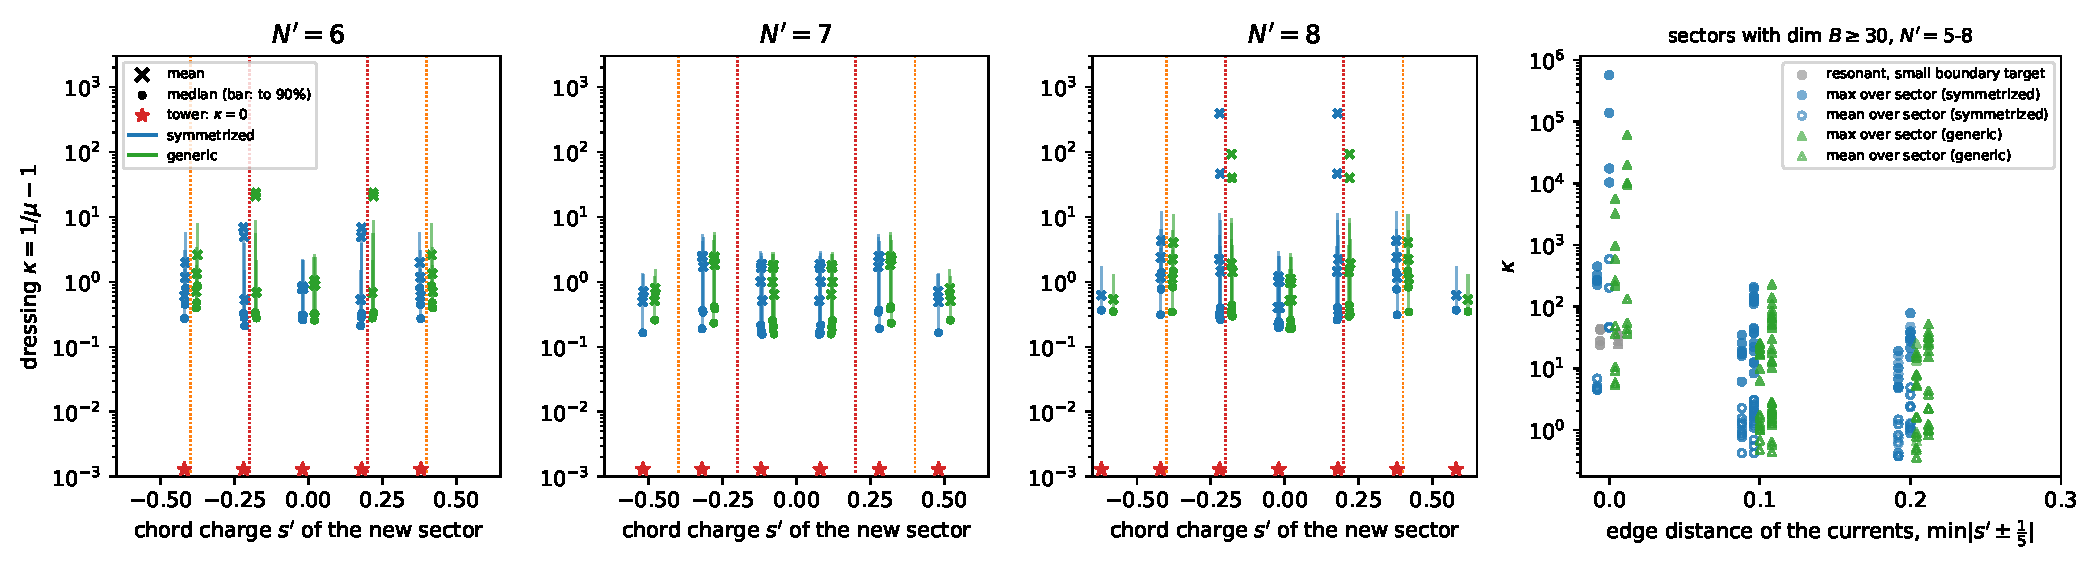
\includegraphics[width=\textwidth]{progress_2026-10-25_figs/fig_resonance.pdf}
\caption{\textbf{Dressing resonances.} Left three panels: exact dressing $\kappa=1/\mu-1$ of the new BPS states, per
sector, vs the sector's chord charge $\sn$, at $\Np=6,7,8$. Marks: crosses = mean, dots = median, bars = median to 90\%;
blue = symmetrized, green = generic. Red dotted lines: $J$-resonant charges $\sn=\pm\tfrac15$. Orange: $z_{11}$-resonant
charges $\pm\tfrac25$. Red stars: the tower, with $\kappa=0$ exactly (drawn at the bottom). Right: largest (filled) and
mean (open) dressing per bulk sector against the distance $\min|\sn\pm\tfrac15|$ of the currents' targets from their
gapless edges, $\Np=5$--8.}
\label{fig:resonance}
\end{figure}

%=====================================================================
\section{Gravitons do not dress}\label{sec:tower}
%=====================================================================

\subsection{Cancellation by a twisted chord}

\DER\ The Ward identity gives $J_{10}=J_{01}=0$ for the tower, at every coupling and every $N$ \cite{prog1023}. In chord
language:
\begin{itemize}\itemsep1pt
\item The cancellation is between the $E$-emission of the 00 slot and the $K$-emission of the 11 slot.
\item Their interference term is the twisted $E$--$K$ matter chord of Proposition~\ref{prop:twisted}(3), i.e.\ a $V$
  insertion.
\item It cancels the direct terms only along a chain $h_{00}\propto Vh_{11}$, $h_{11}\propto Vh'$, \dots\ that ends on a
  state annihilated by $E$. For the tower that state is $\Om$.
\item Black-hole states are not $V$-descendants of $E$-annihilated states, and on them twisted chords are $O(1/N)$
  (Proposition~\ref{prop:twisted}(1)). Their emissions therefore add.
\end{itemize}

\INTERP\ In CCSY's terms, $V$ is the graviton and the tower a multi-graviton state on the vacuum. The new flavor pair
couples to the gravitons only through a symmetry, the $V$ Ward identity, so no dynamics is excited.

\subsection{Tests}

\NUM\ (Fig.~\ref{fig:tower}a.)
\begin{itemize}\itemsep1pt
\item \emph{Each term alone.} The tower's individual emissions $E\Psi_{00}$ and $K\Psi_{11}$ (and $K^\dagger\Psi_{00}$,
  $E^\dagger\Psi_{11}$) are as large as the black-hole averages of the same operators. G-weighted, they lie along the
  diagonal.
\item \emph{At the resonance} they share the enhancement. At $N=7$ (seed~1) the tower's $E$- and $K$-terms into the
  gapless sector $(4,2)$ are 16.9 and 28.2 per unit norm. The black-hole means of the same operators are 61.5 and 21.5.
  The tower's emissions into off-edge targets are 0.02--0.9.
\item \emph{Total.} The currents cancel to $\le2.5\times10^{-16}$, relative to the size of either term.
\item \emph{Isolation.} Outside the window, from $\Np=9$ on, the tower is the unique BPS state in its sector
  (\S\ref{sec:windowtests}). The continuum there is gapped, by \eqref{eq:edges}.
\item \emph{No twisted coherence for black holes} (Fig.~\ref{fig:tower}c).
  \begin{itemize}\itemsep1pt
  \item Take the mean squared $G$-cosine between the $E$-emission of $B(n,n)$ and the $K$-emission of $B(n-1,n-1)$, with
    the tower projected out of both.
  \item It is the same in the two models at every $(N,n)$, for $N=4$--7 and three seeds. For example, it is $0.0064$
    (symmetrized) vs $0.0065$ (generic) at $N=7$, $n=4$, and $0.0219$ vs $0.0210$ at $N=6$, $n=4$.
  \item In the bulk it falls with $N$: 0.044 at $N=5$, 0.006--0.010 at $N=7$.
  \item The tower's own $\cos^2$ is $1$ to $10^{-15}$.
  \item So the symmetrization adds coherence exactly on the $V$-chain and nowhere else, as
    Proposition~\ref{prop:twisted} says.
  \end{itemize}
\end{itemize}

\subsection{Absorbing the new pair}\label{sec:pairing}

\DER+\NUM\ The chord weights factorize by flavor. A black-hole state therefore carries the new $\psi_e$ and $\chi_f$
almost independently:
\[
c\equiv\langle n_{\psi_e}n_{\chi_f}\rangle-\langle n_{\psi_e}\rangle\langle n_{\chi_f}\rangle\approx0 .
\]
The tower $V^n\Om=\sum_S\prod_{i\in S}\psi_i^\dagger\chi_i^\dagger\Om$ is a uniform superposition of $n$ pairs on $\Np$
sites. It carries the new site either empty or doubly occupied, with $c=n(\Np-n)/\Np^2$.

Measured at $\Np=4$--8, in both models:
\begin{itemize}\itemsep1pt
\item The sector means of $c$ over fortuitous states lie in $[-0.023,0.021]$, and in $[-0.002,0.008]$ at $\Np=8$. The
  tower has $c_{\rm tower}=0.11$--$0.25$ (Fig.~\ref{fig:tower}b).
\item Per state, 5--95\% of fortuitous states lie within $\pm0.1$, a range that shrinks with $N$.
\item In bulk sectors, $\langle n_{\psi_e}\rangle$ equals $A/\Np$ to within 0.035.
\item The symmetrized model's fortuitous states carry a slightly larger $c$: the median of the sector means is 0.008 at
  $\Np=7$ and 0.002 at $\Np=8$, against 0.003 and 0.0007 for generic couplings. This is the size expected of an $O(1/N)$
  twisted-chord effect, two orders of magnitude below the tower.
\end{itemize} The 23 October report found tower slot weights $(\Np-n)/\Np$ in 00
and $n/\Np$ in 11, with nothing in 10 or 01. These are just the probabilities that the new site is empty or holds a pair:
graviton counting.

\begin{figure}[t]
\centering
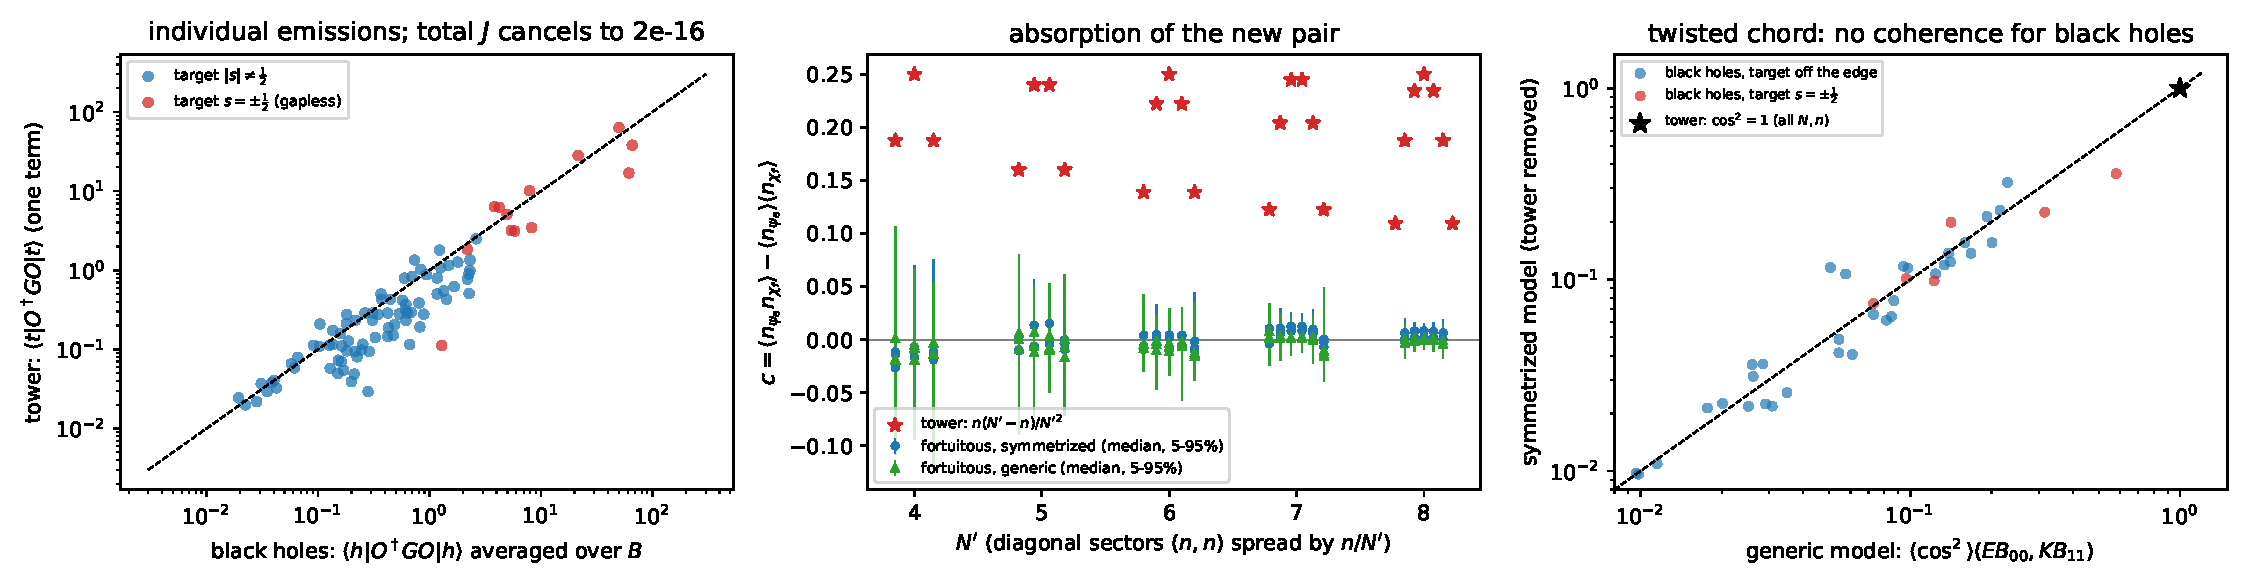
\includegraphics[width=\textwidth]{progress_2026-10-25_figs/fig_tower.pdf}
\caption{\textbf{The tower vs black holes.} (a) Each G-weighted emission of the tower (one term of $J_{10}$ or $J_{01}$,
unit-norm tower state) against the black-hole average of the same operator over the old BPS space. Red: targets on a
gapless edge. In every case the full current cancels to $\le2.5\times10^{-16}$. (b) Connected occupation correlator $c$
of the new pair in diagonal sectors $(n,n)$: fortuitous states (median and 5--95\% range over states) vs the tower (stars,
$n(\Np-n)/\Np^2$). (c) Mean squared $G$-cosine between black-hole $E$- and $K$-emissions, tower removed: symmetrized vs
generic ($N=4$--7, seeds 1--3, every rung). The star is the tower.}
\label{fig:tower}
\end{figure}

%=====================================================================
\section{Monotone versus fortuitous: a chord dictionary}\label{sec:summary}
%=====================================================================

Table~\ref{tab:summary} lists how the chord picture treats the two classes. Every fortuitous entry is derived or tested in
\S\S\ref{sec:window}--\ref{sec:emission}, and every monotone entry in \S\ref{sec:tower}. The two classes differ at each
level:
\begin{itemize}\itemsep1pt
\item where the states live;
\item whether they emit matter chords when the system grows;
\item whether the symmetrization's twisted chords act on them coherently;
\item how they absorb the new flavor pair.
\end{itemize}
The resonances make the contrast sharpest. In the resonant sectors the black holes' dressing is largest, while the tower
in the same sectors stays exactly bare.

\begin{table}[!ht]
\centering\small
\begin{tabular}{p{3.6cm}p{5.4cm}p{5.4cm}}
\toprule
 & fortuitous (black hole) & monotone (tower, graviton gas)\\
\midrule
chord object & zero-length wormhole, $|s|<\tfrac12$ & $V$-descendant of $\Om$; outside the window: alone, gapped\\
where & band \eqref{eq:band} around CCSY's line & diagonal $N_\psi=N_\chi$, crossing the band\\
uplift & emission of chiral matter chords $E,K,Z$ into the window continuum & no emission: $J_{10}=J_{01}=0$\\
obstruction weight & ASC point mass \eqref{eq:pm} & cancelled by the 11 slot\\
dressing & time-integrated ASC two-point function; diverges at gapless edges (resonances at $\sn=\pm\frac15$) & 0 at every $N$, including resonant sectors\\
symmetrization (twisted chords) & $O(1/N)$: identical to the generic model & $O(1)$: the cancelling $V$ insertion\\
$E$--$K$ emission coherence & $\langle\cos^2\rangle\lesssim0.04$, same in both models & $\cos^2=1$\\
absorption of the new pair & independent: $c\approx0$ & bound pair: $c=n(\Np-n)/\Np^2$\\
\bottomrule
\end{tabular}
\caption{The two classes in the chord picture.}
\label{tab:summary}
\end{table}

%=====================================================================
\section{Discussion}\label{sec:discussion}
%=====================================================================

\subsection{Does the distinction emerge in the chord picture?}

Largely yes, with one gap.
\begin{itemize}\itemsep2pt
\item \emph{From the chord rules alone} we get the following.
  \begin{itemize}\itemsep1pt
  \item Where the black holes are: the window and its gapless edges.
  \item How they lift: emission of chiral matter chords into the window continuum, with Al-Salam--Chihara weights and
    resonances at the edges.
  \item That the symmetrization does nothing to them: twisted chords are $O(1/N)$.
  \item That they absorb the new pair flavor by flavor.
  \end{itemize}
  Each of these is tested against the exact finite-$N$ model, in both models.
\item \emph{The tower appears in the chord picture as an exception to each statement.}
  \begin{itemize}\itemsep1pt
  \item It sits outside the window.
  \item It emits nothing, although each of its emissions taken alone is black-hole-sized.
  \item For it, twisted chords are $O(1)$ and supply exactly the cancelling term.
  \item It absorbs the pair bound.
  \end{itemize}
\item \emph{What is not yet chord-intrinsic} is the reason the tower is an exception. Its zero emission is the $V$ Ward
  identity of the microscopic theory. The chord picture identifies the cancelling term as a twisted chord, i.e.\ a
  graviton insertion, and shows why black holes cannot use it, but it does not derive the identity from chord dynamics.
  Doing so needs a chord Hilbert space for graviton states (open problem~2).
\end{itemize}

\subsection{What is established, and how firmly}
\begin{itemize}\itemsep2pt
\item \DER\ The dictionary (Proposition~\ref{prop:dict}, eqs.~\eqref{eq:delta}--\eqref{eq:deltas}), the exact chirality
  \eqref{eq:chiral}, the twisted-chord counting (Proposition~\ref{prop:twisted}), the window and its gapless edges, and the
  resonance positions. The derivations are double-scaled ($p\to\infty$), like BBNR's.
\item \NUM\ The dictionary works at $p=(2,1)$ and $N\le10$:
  \begin{itemize}\itemsep1pt
  \item the support of the BPS sectors;
  \item obstruction weights to 5--20\%;
  \item dressing integrals to within a factor of about 1.4;
  \item continuum edges to within a factor of about 1.5;
  \item gaps collapsing at the window edge;
  \item resonances where predicted, in both models;
  \item the tower's individual emissions BH-like, with total zero;
  \item no twisted coherence on black holes;
  \item pairing.
  \end{itemize}
\item \INTERP\ The gravitational reading. Zero-length wormholes are black holes and the window edges are the $Q=\pm\frac12$
  supermultiplets of the super-Schwarzian. The tower is a graviton gas that the enlarged system dresses only through a
  symmetry.
\end{itemize}

\subsection{Limitations}
\begin{itemize}\itemsep1pt
\item The chord theory is double-scaled, while the model has $p_\chi=1$ and $N\le10$. The residual scatter of the
  dictionary is of the size seen in the one-flavor model, but somewhat larger.
\item The resonance is a statement about the upper tail. Means and maxima respond strongly; medians do not.
\item The mean exact dressing is not yet predicted sector by sector from chords, because that needs the slot weights of
  the new BPS states and their interference. We test the building blocks and the positions of the divergences.
\item The chord theory of graviton states, with twisted chords at $O(1)$, is not built. The tower's protection is
  derived from the Ward identity, and only read in chord language.
\end{itemize}

\subsection{Open problems}
\begin{enumerate}\itemsep2pt
\item \emph{The exact uplift from chords.} The transfer $\Zc$ and the leak maps $\alpha,\gamma$ of \cite{prog1023} are
  products of the same matter chords with $Q_0^+$. They are uncrossed diagrams and should be computable like the
  self-energies.
\item \emph{A Hilbert space for graviton states.} Can twisted chords be resummed into a chord Hilbert space whose zero
  modes are the tower states? This would derive the protection within the chord theory itself.
\item \emph{Large $N$.} From $\Np=6$ to 8 the resonance grew by one to two orders of magnitude, following the edge gap.
  The edge gap stalls at $N=9$, so whether the resonant dressing keeps growing at $\Np=10$ (resonant parity) is open.
  The test needs sparse methods for the new model. So does the question whether the stall is a finite-$p$ offset of the
  edge or a genuine finite-$N$ gap.
\item \emph{The decoder.} Does the project's main object, the compressed slot projector, inherit the window structure?
  One would expect black-hole sectors to give its Jacobi-type bulk, and the tower to sit apart on the pairing line
  $c=n(\Np-n)/\Np^2$. This is not tested here.
\end{enumerate}

\appendix

%=====================================================================
\section{Verification summary}\label{app:verify}
%=====================================================================

\begin{table}[ht]
\centering\small
\begin{tabular}{p{7.2cm}p{7.6cm}}
\toprule
check & result\\
\midrule
\multicolumn{2}{l}{\emph{\texttt{tests/test\_two\_flavor\_chords.py} (6 tests, all pass)}}\\
charge bookkeeping: $Q$ raises $s$ by 1, $V$ by $\tfrac15$; $\delta_{E,K,Z}=\tfrac35,\tfrac45,\tfrac25$; particle--hole $s\to-s$ & exact\\
dressing targets of the six terms follow the slot equations; resonance positions & exact\\
every non-tower BPS sector at $\Np=6$ lies in $|s|\le\tfrac12$ (both models) & pass\\
$\Np=9$, sector $(1,1)$: one BPS state (symmetrized), none (generic) & pass\\
window-edge gap collapses at $N=7$: $(4,2)$ gap $<10^{-3}$ of mean; $(4,4)$ gap $>10^{-2}$ & pass\\
obstruction weight of $Z$ from $(3,4)$, $N=6$, vs chord point mass & within 10\%\\
\multicolumn{2}{l}{\emph{\texttt{tests/test\_two\_flavor.py} (21 tests of the 23 October report, rerun)}}\\
block form, identities, slot equations, Theorem~1, dimension formulas, tower, closed forms & all pass\\
\multicolumn{2}{l}{\emph{checks inside the runs}}\\
$[E,K]=0$, $\{Q_0,Z\}=0$ (both models, $N=4$) & $\le1.8\times10^{-15}$ (entries $O(10)$)\\
tower currents $J_{10}$, $J_{01}$ (all rungs, $N=3$--7, seeds 1--3) & $\le2.5\times10^{-16}$ relative\\
tower $\cos^2$ between its $E$- and $K$-emissions (twisted task) & $1-O(10^{-15})$\\
optimized spectra vs full diagonalization ($\Np=7$) & identical BPS counts; gaps, means to $1.7\times10^{-12}$\\
\bottomrule
\end{tabular}
\caption{Verification.}
\end{table}

%=====================================================================
\section{Numerical methods and reproducibility}\label{app:repro}
%=====================================================================

\paragraph{Model and couplings.} Everything follows the 23 October report \cite{prog1023}. The couplings $C_1$ of the
$(N+1)$-pair model are drawn by \texttt{random\_symmetric\_couplings} (or \texttt{random\_generic\_couplings}) with
\texttt{numpy.random.default\_rng(seed)}, and the old model is their restriction to the first $N$ pairs. So ``old $N$, seed $s$'' is the same realization there and
here. The window task draws an $\Np$-pair model at size $\Np$ with the same rule.

\paragraph{Exact quantities.}
\begin{itemize}\itemsep1pt
\item \emph{BPS counts and gaps} come from the Gram matrices of the two $Q$ maps of each sector. The Laplacian is their
  direct sum plus the BPS kernel.
\item \emph{The dressing building blocks} are exact averages over unit-variance independent couplings of
  $\Tr(P_H O^\dagger G O P_H)/b$, estimated with six random-phase draws. The string-diagonal part is exact and the cross
  terms average out; statistical errors are recorded per block.
\item \emph{Exact dressings} $\kappa=1/\mu-1$ use the exact bare-fraction spectrum $\mu$ of the new BPS space (23 October
  report, \S\S6, 9).
\end{itemize}

\paragraph{Chord quantities.}
\begin{itemize}\itemsep1pt
\item The ASC weight of \texttt{src/dssyk\_n2.py} (14 October report) is evaluated at $(\lambda,s,\delta)$ from
  \eqref{eq:dict}--\eqref{eq:deltas}, with Gauss--Legendre quadrature in $\phi$ (2001 nodes).
\item The energy scale is $\kappa=m_1/(q^s+q^{-s})$, with $m_1$ the exact mean Laplacian eigenvalue of the target
  sector.
\item There are no fitted parameters.
\end{itemize}

\paragraph{Runs.} All runs used \texttt{scripts/run\_two\_flavor\_chords.py} under \texttt{scripts/memwatch.py}, with
outputs in \texttt{results/data/two\_flavor\_chords\_2026-10-25/}.

\begin{center}\footnotesize
\begin{tabular}{lp{4.6cm}lll}
\toprule
job & tasks & sizes & seeds, models & peak\\
\midrule
small & blocks, tower, resonance, pairing; window & $N=3$--6; $\Np=4$--7 & 1--3, both & 0.19 GB\\
N7 sym & tower, blocks, resonance, pairing & $N=7$ & 1--2, sym & 2.55 GB\\
N7 generic & blocks, resonance, pairing & $N=7$ & 1--2, generic & 2.70 GB\\
window & window & $\Np=8$; $\Np=9,10$ ($\dim\le3000$) & 1--2, both & 2.11 GB\\
edge gap & edgegap & $N=3,5,7$; $N=9$ & 1--3; 1--2, both & 6.8 GB\\
twisted & twisted & $N=4$--7 & 1--3, both & 0.25 GB\\
\bottomrule
\end{tabular}
\end{center}
The first attempt at the window job, with an unoptimized eigensolver, was stopped by hand before it wrote any
record (peak 1.75 GB). The generic $N=9$ edge gaps ran as two parallel jobs (peaks 6.8 GB each; about 30 minutes per
diagonalization on one core). The estimates of \texttt{--dry-run} (4.9 GB at $N=7$) were conservative. Figures and
\texttt{summary.json}: \texttt{scripts/analyze\_two\_flavor\_chords.py}. Tests:
\texttt{.venv/bin/python tests/test\_two\_flavor\_chords.py} (6) and \texttt{tests/test\_two\_flavor.py} (21).

\begin{thebibliography}{99}\small
\bibitem{CV} J.~Chryssanthacopoulos and D.~Vegh, \emph{Fortuity and fragility in supersymmetric SYK}, arXiv:2608.12160 (2026).
\bibitem{CCSY} C.-M.~Chang, Y.~Chen, B.~S.~Sia and Z.~Yang, \emph{Fortuity in SYK models}, arXiv:2412.06902.
\bibitem{HTZ} M.~Heydeman, G.~J.~Turiaci and W.~Zhao, \emph{Phases of $\mathcal N=2$ Sachdev-Ye-Kitaev models}, arXiv:2206.14900.
\bibitem{BBNR} M.~Berkooz, N.~Brukner, V.~Narovlansky and A.~Raz, \emph{The double scaled limit of super-symmetric SYK models}, JHEP 12 (2020) 110, arXiv:2003.04405.
\bibitem{BLY} J.~Boruch, H.~W.~Lin and C.~Yan, \emph{Exploring supersymmetric wormholes in $\mathcal N=2$ SYK with chords}, arXiv:2308.16283.
\bibitem{HITZ} M.~Heydeman, L.~V.~Iliesiu, G.~J.~Turiaci and W.~Zhao, \emph{The statistical mechanics of near-BPS black holes}, arXiv:2011.01953.
\bibitem{prog1014} \texttt{syk\_gravity} project, \emph{Progress report, 14 October 2026: the dressing spectrum from chords}, \texttt{research/pdfs/progress\_2026-10-14.pdf}.
\bibitem{prog1023} \texttt{syk\_gravity} project, \emph{Progress report, 23 October 2026 (revised 25 October): monotone and fortuitous states in the two-flavor uplift}, \texttt{research/pdfs/progress\_2026-10-23.pdf}.
\end{thebibliography}

\end{document}
